\documentclass[12pt, a4paper]{article}

% Russian-specific packages
\usepackage[T2A]{fontenc}
\usepackage[utf8]{inputenc}
\usepackage[russian,english]{babel}

% Graphics
\usepackage{graphicx}
\DeclareGraphicsExtensions{.pdf, .png, .jpg}
\usepackage{wrapfig}

% Color text
% Remove for release
\usepackage{color}

% Same line width
\sloppy

% Setup captions for figures
\usepackage{caption}

% Enumerate item 
\usepackage[shortlabels]{enumitem}

%Math packages
\usepackage{amsmath}

% Subfigures
\usepackage{subfig}

% Hyperlink
\usepackage{hyperref}
\hypersetup{
    colorlinks=true,
    linkcolor=black,
    filecolor=magenta,
    citecolor=black,      
    urlcolor=black,
    pdftitle={Database},
    pdfpagemode=FullScreen,
}

% Содержание
\addto\captionsenglish{\renewcommand{\contentsname}{\begin{center}СОДЕРЖАНИЕ\end{center}}}

\newcommand{\comment}[1]{\textcolor{red}{#1}}

\begin{document}
    \tableofcontents

    \section{Введение}

    Задачи экологии имеют первостепенное значние. Важно научиться применять методы для анализа математических моделей различных экологических систем. 
    
    Одна из основных задач экологии --- изучение структуры системы и то, как она функционирует, поиск закономерностей. В качестве инструмента для анализа систем можно использовать методы из различных разделов математики, в частности нелинейеной динамики.
    
    В данной работе предложены некоторые выкладки по анализу дискретной модели Хасселя. Подобные модели широко используется в качестве общих моделей динамики популяции с дискретным временем и наличием конкуренции за ресурсы и внутривидовой конкуренции. Так же их используют для исследования различных явлений в динамике популяций.

    \comment{Нврн у нас есть эффект Алли. Только пока про это нет ни слова.}

    \comment{https://royalsocietypublishing.org/doi/10.1098/rsos.182178\#d3e228}

    \comment{https://www.hindawi.com/journals/ddns/2020/8148634/}

    \comment{https://www.jstor.org/stable/3863}

    \comment{https://www.imperial.ac.uk/people/m.hassell/publications.html}

    

    \newpage

    \section{Детерминированная модель}

    \subsection{Описание модели}

    Одна из вариаций модели Хасселя \cite{densityDependenceInSingleSpeciesPopulations} имеет следующую математическая запись:

    \begin{equation}
        \label{origin}
        x_{t+1} = \frac{\alpha x_t^2}{(\beta + x_t)^6}.
    \end{equation}

    В данной формуле \(x_t\) --- количество особей в поколении с номером \(t\). Параметр \(\alpha\) определяет скорость роста популяции, а параметр \(\beta\) определяет несущую способность окружающей среды.
    
    Для упрощения задачи рассмотрим частный случай. Зафиксируем параметр \(\alpha = 1\). Параметр \(\beta\) изменяется в диапазоне \([0; 0.6]\). Для нахождения равновесий требуется решить следующее уравнение:  

    \[x = \frac{\alpha x^2}{(\beta + x)^6}\]
    
    \[1 = \frac{\alpha x}{(\beta + x)^6}\]

    \begin{equation}
        \label{baseEquation}
        \alpha x = (\beta + x)^6
    \end{equation}

    Построим графики функций \(y = \alpha x\) и \(y = (\beta + x)^6\). 
        
    В зависимости от значений параметра \(\beta\) уравнение (\ref{baseEquation}) может иметь ноль (при \(\beta > 0.582355932\)), один (при \(\beta \approx 0.582355932\)) или два корня (при \(\beta < 0.582355932\)). На рисунках \ref{mainIntersect}, \ref{mainTouch} и \ref{mainOver} можно увидеть все возможные варианты. При \(\beta=0.582355932\) в модели наблюдается касательная бифуркации, сопровождающаяся появлением двух равновесий (см. рис. \ref{mainTouch}).

    \begin{figure}
        \centering
        \subfloat[\(\beta = 0.57\)]{
            \label{mainIntersect}
            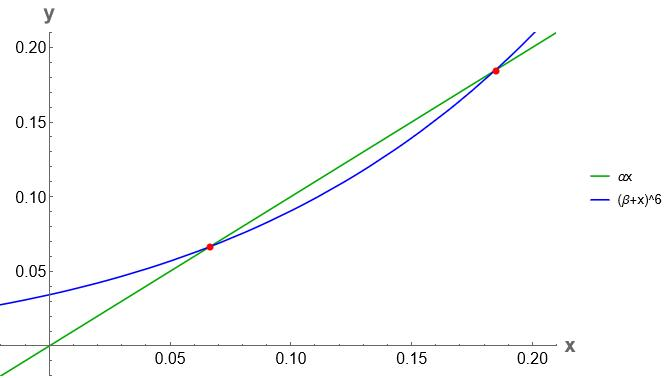
\includegraphics[width=0.5\textwidth]{deterministic/images/two_intersection.jpg}
        }
        \subfloat[\(\beta \approx 0.582355932\)]{
            \label{mainTouch}
            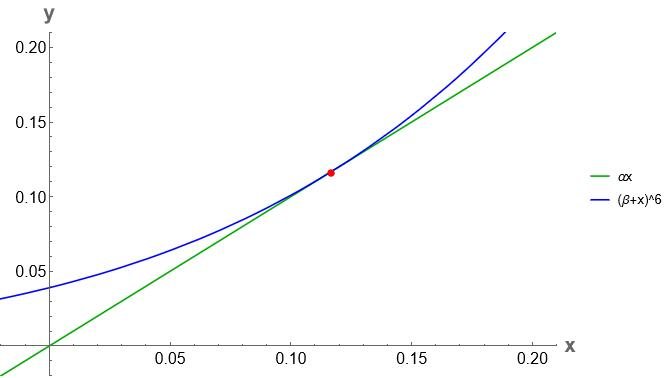
\includegraphics[width=0.5\textwidth]{deterministic/images/one_intersection.jpg}
        }

        \subfloat[\(\beta = 0.59\)]{
            \label{mainOver}
            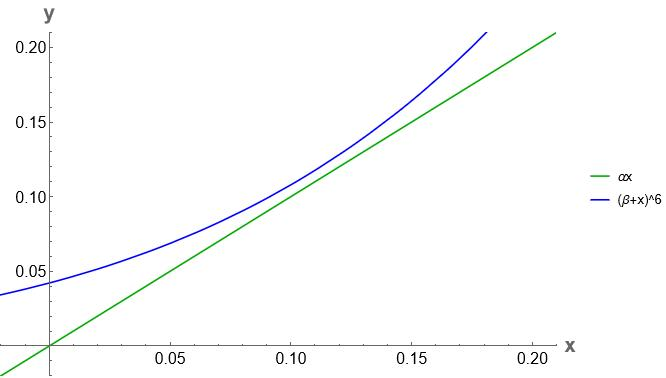
\includegraphics[width=0.5\textwidth]{deterministic/images/zero_intersection.jpg}
        } 
        % Было 0.75

        \captionsetup{justification=centering}
        \caption{Решения уравнения (\ref{baseEquation}) для разных значений параметра \(\beta\)}
    \end{figure}
  
        
    \subsection{Временные ряды}

        На временных рядах можно продемонстрировать как различные виды шума влияют на поведение системы.

        На рисунке \ref{time_series_x_0_06_a_1_b_0_56} изображено поведение модели без добавления каких-либо шумов. Видно, что значения переменной \(x\) с течением времени стабилизируются. Численность популяции фактически остается неизменной.

        \begin{figure}
            \centering
            \subfloat[Для модели (\ref{origin})]{
                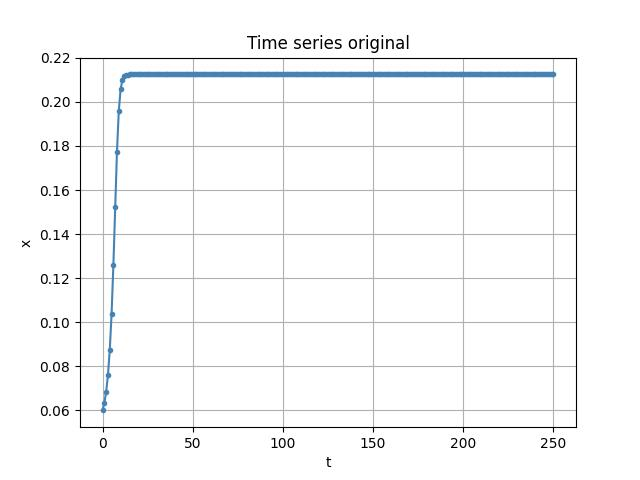
\includegraphics[width=0.5\textwidth]{stochastic/time_series_x_0_06_a_1_b_0_56.jpg}
                \label{time_series_x_0_06_a_1_b_0_56}
            }
            \subfloat[Для модели (\ref{alpha_chaos})]{
                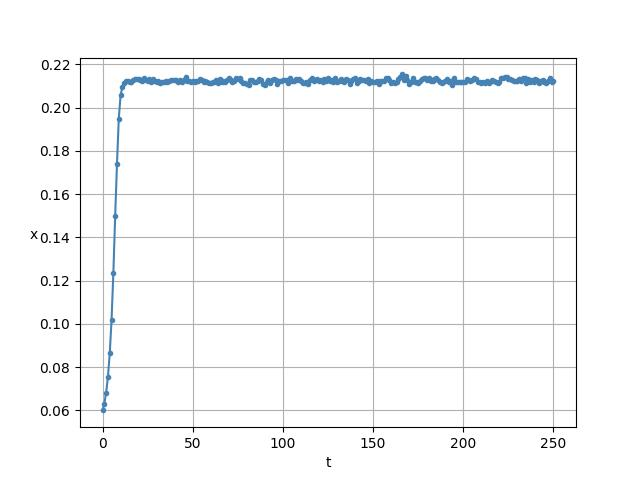
\includegraphics[width=0.5\textwidth]{stochastic/time_series_x_0_06_a_1_b_0_56_alpha_chaos_epsilon_0_004.jpg}
                \label{time_series_x_0_06_a_1_b_0_56_alpha_chaos_epsilon_0_004}
            }  

            \subfloat[Для модели (\ref{beta_chaos})]{
                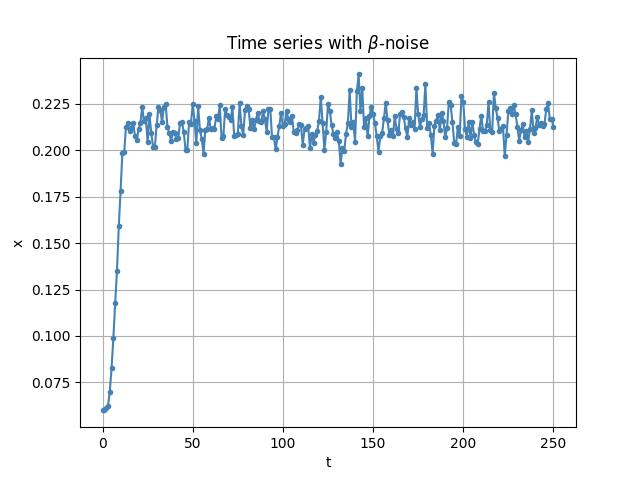
\includegraphics[width=0.5\textwidth]{stochastic/time_series_x_0_06_a_1_b_0_56_beta_chaos_epsilon_0_004.jpg}
                \label{time_series_x_0_06_a_1_b_0_56_beta_chaos_epsilon_0_004}
            }
            \subfloat[Для модели (\ref{additive_chaos})]{
                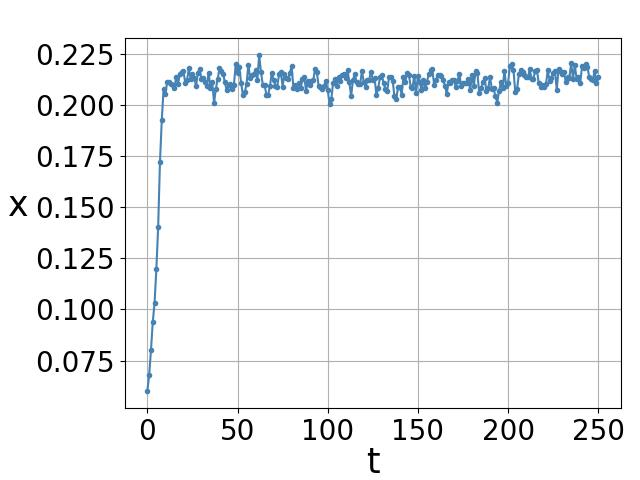
\includegraphics[width=0.5\textwidth]{stochastic/time_series_x_0_06_a_1_b_0_56_additive_chaos_epsilon_0_004.jpg}
                \label{time_series_x_0_06_a_1_b_0_56_additive_chaos_epsilon_0_004}
            }
            
            \caption{Временные ряды при \(\alpha = 1, \beta = 0.56, x_0 = 0.06, \varepsilon = 0.004\)}
        \end{figure}

        Далее на рисунках \ref{time_series_x_0_06_a_1_b_0_56_alpha_chaos_epsilon_0_004}, \ref{time_series_x_0_06_a_1_b_0_56_beta_chaos_epsilon_0_004}, \ref{time_series_x_0_06_a_1_b_0_56_additive_chaos_epsilon_0_004} представлены временные ряды для различных видов шума: 

        \begin{enumerate}[a)]
            \setcounter{enumi}{1}
            \item \(\alpha\)-шум
            \item \(\beta\)-шум
            \item аддитивный шум
        \end{enumerate}

        Все варианты рассматриваются с одной и той же интенсивностью шума \(\varepsilon = 0.004\). 
        
        Мы видим, что вид шума влияет на величину разброса значений численности популяции. \comment{Приплети сюда дисперсию.} И если раньше численность популяции стабилизировалась и переставала хоть сколько-нибудь меняться, то сейчас численность постоянно всегда колеблется, но как можно заметить, она меняется в рамках некоторого коридора значений. Численность популяции в общем то не растет и не уменьшается на какую-то значительную величину. Но такое поведение наблюдается не всегда.

        \comment{малый шум будет оказывать незначительное влияние, а большой - огромное.}

        \comment{Можно взять оригинальный временной ряд и на него сверху наложить временной ряд с шумом.}

        \comment{Хорошая фраза: индуцированный шумом переход}

        Для того чтоб продемонстрировать другое возможное поведение, давайте увеличим интенсивность шума. Пускай теперь \(\varepsilon = 0.04\). Рассмотрим рисунок \ref{time_series_x_0_06_a_1_b_0_56_beta_chaos_epsilon_0_04_fall}. Здесь мы видим ситуацию, когда шум оказал негативное влияние на численность популяции. Но опять же все не так просто. Если мы еще раз запустим алгоритм, который просчитывает нашу модель, то мы увидим, что популяция успешно выживала на протяжении анализируемого интервала времени. Данный пример проиллюстрирован на картинке \ref{time_series_x_0_06_a_1_b_0_56_beta_chaos_epsilon_0_04_alive}. Аналогичные эффекты можно наблюдать и при других видах шума.

        \comment{Примерно в \(t = 50\) обе популяции были близки к вымиранию, но одна выжила, а вторая нет. "Одно рисовое зернышко может склонить чашу весов" (с) какой-то мультик.}

        \begin{figure}
            \centering
            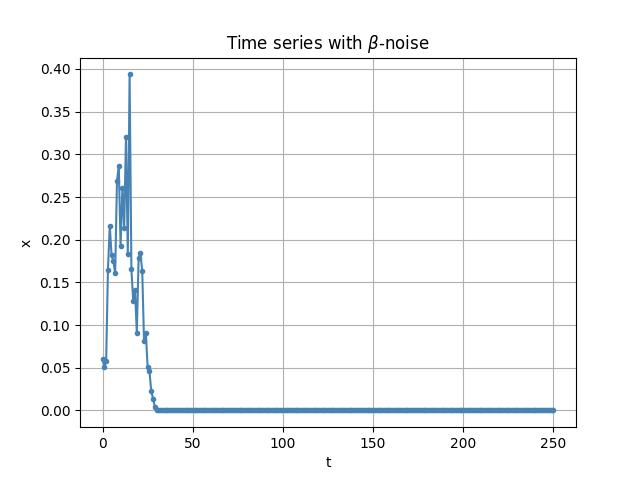
\includegraphics[width=\textwidth]{stochastic/time_series_x_0_06_a_1_b_0_56_beta_chaos_epsilon_0_04_fall.jpg}
        
            \captionsetup{justification=centering}
            \caption{Временной ряд модели (\ref{beta_chaos}) при \(\beta = 0.56, \alpha = 1, x_0 = 0.06, \varepsilon = 0.04\)}
            \label{time_series_x_0_06_a_1_b_0_56_beta_chaos_epsilon_0_04_fall}
        \end{figure}

        \begin{figure}
            \centering
            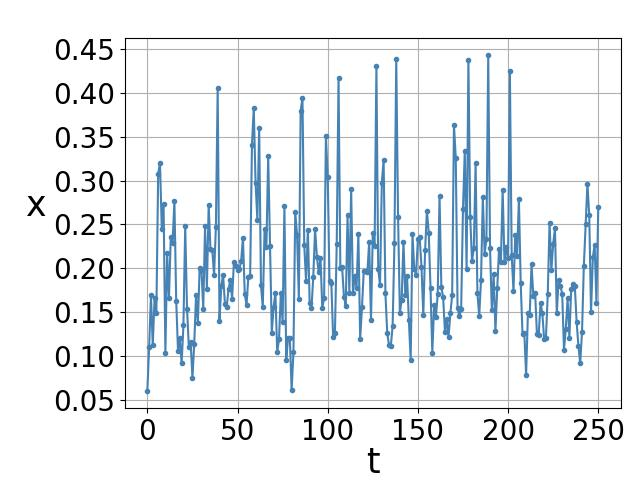
\includegraphics[width=\textwidth]{stochastic/time_series_x_0_06_a_1_b_0_56_beta_chaos_epsilon_0_04_alive.jpg}
        
            \captionsetup{justification=centering}
            \caption{Временной ряд модели (\ref{beta_chaos}) при \(\beta = 0.56, \alpha = 1, x_0 = 0.06, \varepsilon = 0.04\)}
            \label{time_series_x_0_06_a_1_b_0_56_beta_chaos_epsilon_0_04_alive}
        \end{figure}

        Анализируя вышесказанное можно сказать, что при добавлении в модель случайных событий ее поведение становится непредсказуемым. Одно незначительное изменение может кардинально повлиять на ход развития событий. 

        \comment{рассматривать как в том семестре все возможные варианты поведения системы в зависимости от начальной точки думаю не надо и так все понятно.}

    \subsection{Лестница Ламерея}

    Существует также инструмент визуализации решения отображения (\ref{baseEquation}) называемый лестницей Ламерея. Этот метод аналогично временному ряду позволяет иллюстрировать то, как изменяется численность популяции с течением времени.
    
    Опять же рассмотрим подробнее основные типичные ситуации. Для этого зафиксируем параметр: \(\beta = 0.56\). 

    \begin{figure}
        \centering
        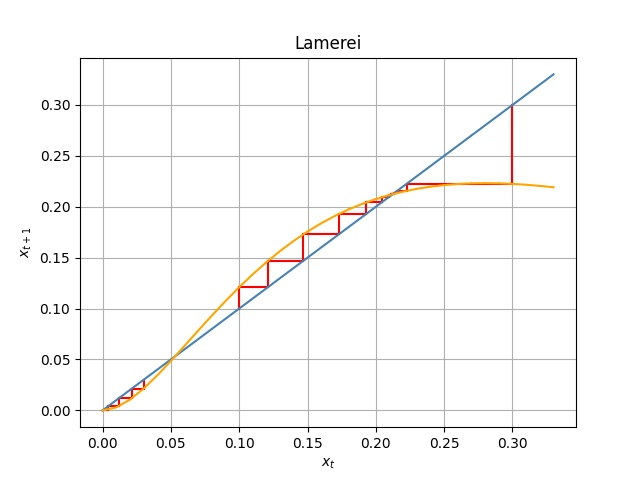
\includegraphics[width=\textwidth]{deterministic/lamerei_b_0_56.jpg}

        \captionsetup{justification=centering}
        \caption{Лестница Ламерея модели (\ref{origin}) для \(\beta = 0.56\) и \(x_0 = 0.03\), \(x_0 = 0.1\) и \(x_0 = 0.3\)}
        \label{lamerei_b_0_56}
    \end{figure}

    Давайте зафиксируем начальную численность популяции \(x_0 = 0.03\). На рисунке \ref{lamerei_b_0_56} мы видим, что траектория сходится к нулю. В биологическом смысле это означает, что популяция с течением времени вымирает.

    А теперь зафиксируем начальную численность популяции на уровне \(x_0 = 0.06\). На рисунке \ref{lamerei_b_0_56} видно, что при таких начальных условиях численность популяции сходится к \(x \approx 0.21\).
    
    Очень похожую ситуацию мы можем наблюдать на рисунке \ref{lamerei_b_0_56}. Такой график построен при начальном значении \(x_0 = 0.3\). Значения численности популяции тоже сходятся к устойчивому равновесию. Численность снова стабилизируется.
    
    Теперь рассмотрим ситуацию, когда начальная численность популяции очень большая. Такая ситуация изображена на рисунках \ref{lamerei_x_1_3_b_0_56} и \ref{lamerei2_x_1_3_b_0_56}. Мы видим, что популяция вымирает.

    \begin{figure}
        \centering
        \subfloat[Общий вид лестницы Ламерея]{
            \label{lamerei_x_1_3_b_0_56}
            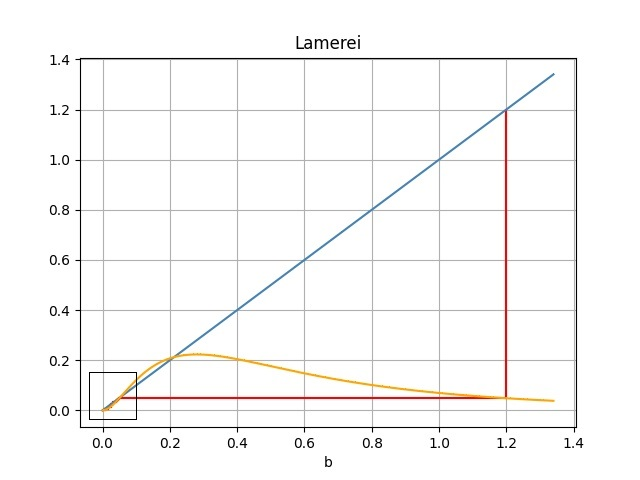
\includegraphics[width=0.9\textwidth]{deterministic/lamerei_x_1_3_b_0_56.jpg}
        }

        \subfloat[Дополнение к \ref{lamerei_x_1_3_b_0_56}]{
            \label{lamerei2_x_1_3_b_0_56}
            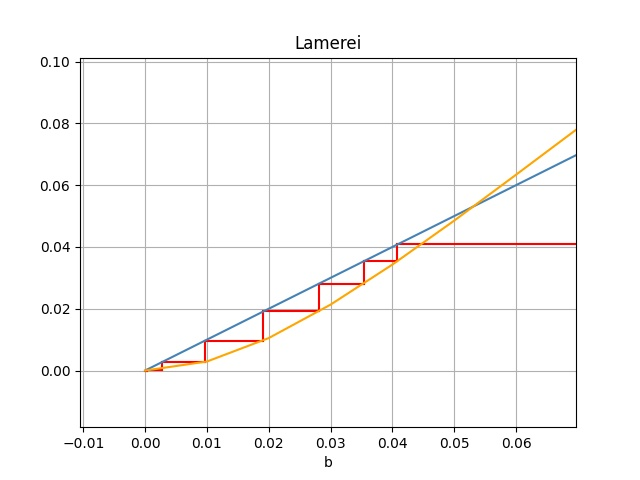
\includegraphics[width=0.9\textwidth]{deterministic/lamerei2_x_1_3_b_0_56.jpg}
        }

        \captionsetup{justification=centering}
        \caption{Лестница Ламерея модели (\ref{origin}) для \(\beta = 0.56\) и \(x_0 = 1.3\)}
    \end{figure}

    Таким образом, кроме маленького порогового значения численности популяции существует еще и большое значение, задающие интервал существования популяции. Вне этого интервала популяция вымирает. 


    \subsection{Стохастические диаграммы}

    Далее представлено влияние случайного возмущения на бифуркационных диаграммах для разных видов шума. На рисунках \ref{bifurcation_x_0_2_a_1_compare_alpha_noise}, \ref{bifurcation_x_0_2_a_1_compare_beta_noise} и \ref{bifurcation_x_0_2_a_1_compare_additional_noise} представлены графики бифуркационных диаграмм для моделей (\ref{alpha_chaos}), (\ref{beta_chaos}) и (\ref{additive_chaos}). Во всех моделях зафиксировано значение параметра \(\alpha = 1\). На каждом графике, так же как и в исходной модели, существует участок равновесия, участки с циклами и участок с хаотическим поведением системы. От вида и интенсивности шума зависит то, насколько выделены участки с регулярной динамикой.

    Видно, что модель с \(\alpha\)-шум сохранят бифуркационную структуру лучше, чем модель с \(\beta\)-шумом и с аддитивным шумом.

    \begin{figure}
        \centering
        \subfloat[для модели (\ref{origin}) (без шума)]{
            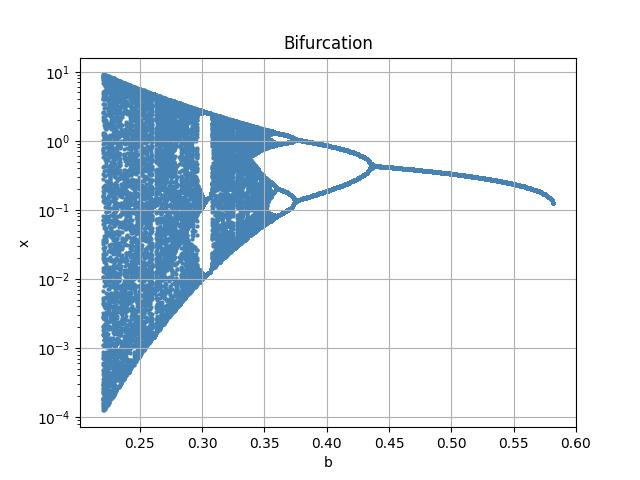
\includegraphics[width=0.55\textwidth]{stochastic/images/bifurcation_x_0_2_a_1_compare_no_noise.jpg}
            \label{bifurcation_x_0_2_a_1_compare_no_noise}
        }  
        \subfloat[для модели (\ref{alpha_chaos}) (с \(\alpha\)-шумом)]{
            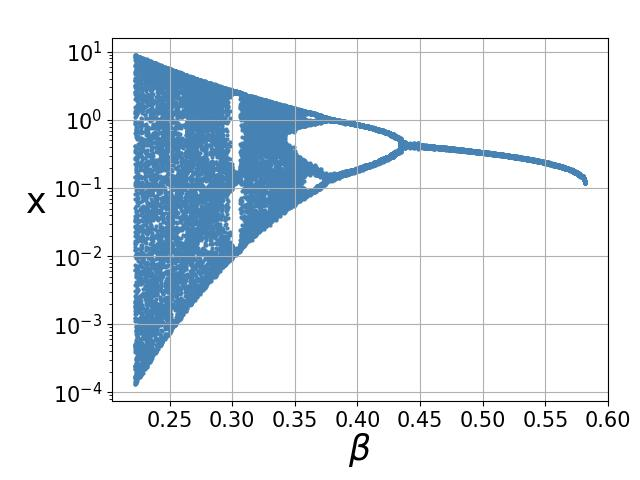
\includegraphics[width=0.55\textwidth]{stochastic/images/bifurcation_x_0_2_a_1_compare_alpha_noise.jpg}
            \label{bifurcation_x_0_2_a_1_compare_alpha_noise}
        }
        
        \subfloat[для модели (\ref{beta_chaos}) (с \(\beta\)-шумом)]{
            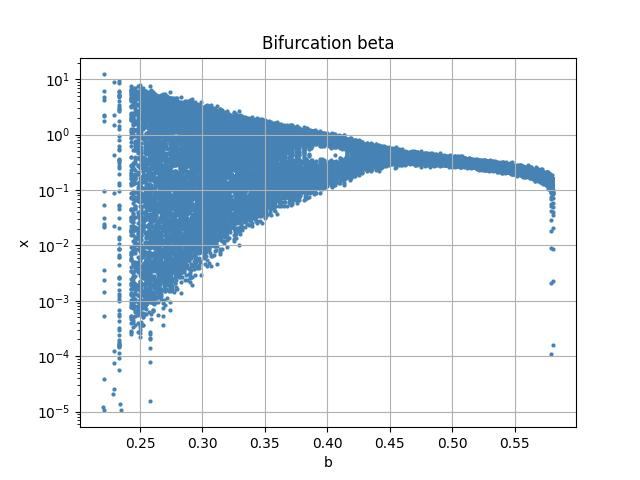
\includegraphics[width=0.55\textwidth]{stochastic/images/bifurcation_x_0_2_a_1_compare_beta_noise.jpg}
            \label{bifurcation_x_0_2_a_1_compare_beta_noise}
        }
        \subfloat[для модели (\ref{additive_chaos}) (с аддитивным шумом)]{
            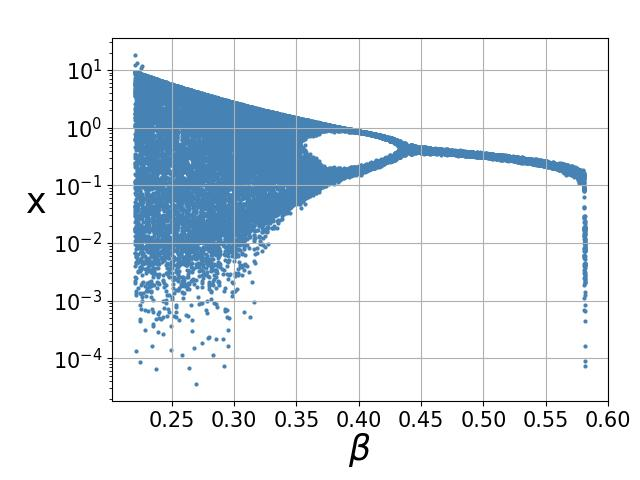
\includegraphics[width=0.55\textwidth]{stochastic/images/bifurcation_x_0_2_a_1_compare_additional_noise.jpg}
            \label{bifurcation_x_0_2_a_1_compare_additional_noise}
        }
            
        \caption{Бифуркационная диаграмма при \(\varepsilon = 0.01\)}
    \end{figure}

    % \begin{figure}
    %     \centering
    %     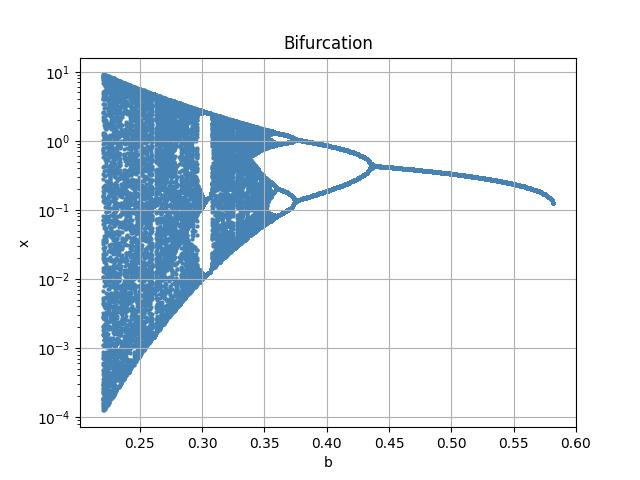
\includegraphics[width=\textwidth]{stochastic/images/bifurcation_x_0_2_a_1_compare_no_noise.jpg}
        
    %     \captionsetup{justification=centering}
    %     \caption{Бифуркационная диаграмма для модели (\ref{origin})}
    %     \label{bifurcation_x_0_2_a_1_compare_no_noise}
    % \end{figure}


    \subsection{Показатель Ляпунова}    

    Для определения устойчивости аттракторов часто используется показатель Ляпунова. Зависимость этого показателя для аттракторов модели (\ref{origin}) представлена на рисунке \ref{lyapunov}. 

    \begin{figure}
        \centering
        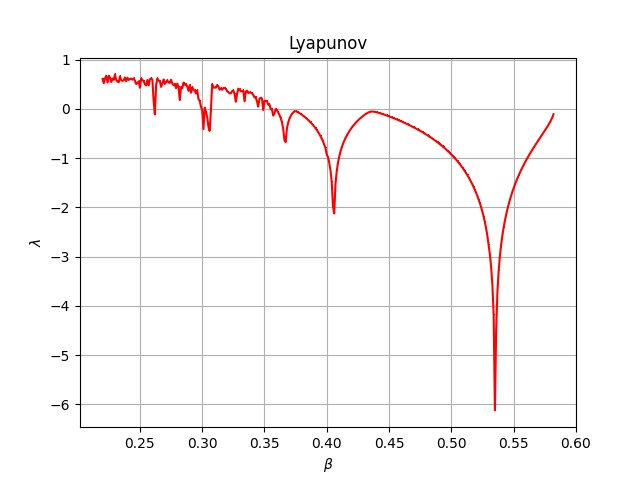
\includegraphics[width=\textwidth]{deterministic/lyapunov.jpg}

        \captionsetup{justification=centering}
        \caption{Показатель Ляпунова для модели (\ref{origin})}
        \label{lyapunov}
    \end{figure}

    На этом графике мы видим, что точки, где график показателя Ляпунова касается нуля точно соответствуют бифуркционным значениям, которые можно наблюдать на бифуркационной диаграмме представленной на рисунке \ref{bifurcation}.

    \subsection{Карта режимов}

    Карта режимов, представленная на рисунке \ref{regimeMap}, позволяет показать возникающие динамические режимы системы при определенных значениях параметров \(\alpha\) и \(\beta\).

    Можно заметить, что при любом значении параметра \(\alpha\) существует каскад бифуркации удвоения периода при уменьшении параметра \(\beta\). Чем меньше параметр \(\alpha\), тем меньше интервал значений параметра \(\beta\), при котором этот каскад существует. После его исчезновения аттрактором системы является только равнвовесие \(\bar{x}_1\).

    \begin{figure}
        \centering
        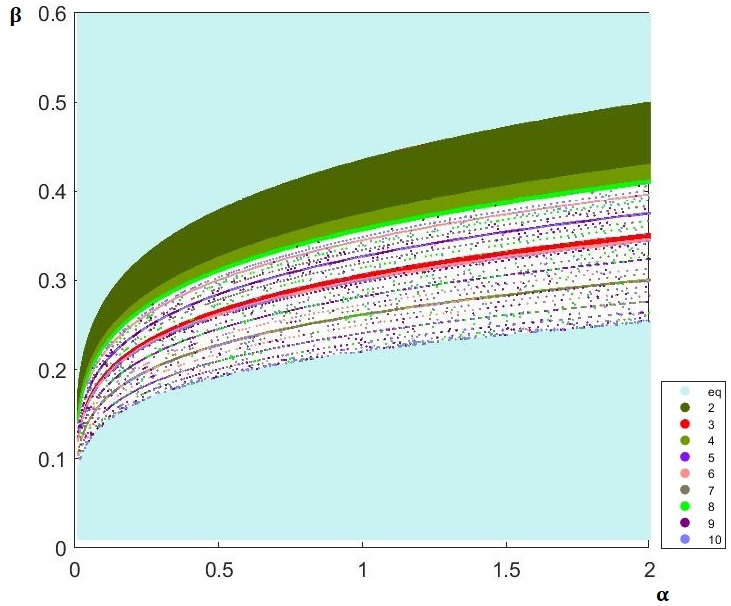
\includegraphics[width=\textwidth]{deterministic/regime_map.jpg}

        \captionsetup{justification=centering}
        \caption{Карта режимов модели (\ref{origin})}
        \label{regimeMap}
    \end{figure}



    \newpage

    \section{Стохастическая модель}

    \subsection{Описание модели}

    Одна из вариаций модели Хасселя \cite{densityDependenceInSingleSpeciesPopulations} имеет следующую математическая запись:

    \begin{equation}
        \label{origin}
        x_{t+1} = \frac{\alpha x_t^2}{(\beta + x_t)^6}.
    \end{equation}

    В данной формуле \(x_t\) --- количество особей в поколении с номером \(t\). Параметр \(\alpha\) определяет скорость роста популяции, а параметр \(\beta\) определяет несущую способность окружающей среды.
    
    Для упрощения задачи рассмотрим частный случай. Зафиксируем параметр \(\alpha = 1\). Параметр \(\beta\) изменяется в диапазоне \([0; 0.6]\). Для нахождения равновесий требуется решить следующее уравнение:  

    \[x = \frac{\alpha x^2}{(\beta + x)^6}\]
    
    \[1 = \frac{\alpha x}{(\beta + x)^6}\]

    \begin{equation}
        \label{baseEquation}
        \alpha x = (\beta + x)^6
    \end{equation}

    Построим графики функций \(y = \alpha x\) и \(y = (\beta + x)^6\). 
        
    В зависимости от значений параметра \(\beta\) уравнение (\ref{baseEquation}) может иметь ноль (при \(\beta > 0.582355932\)), один (при \(\beta \approx 0.582355932\)) или два корня (при \(\beta < 0.582355932\)). На рисунках \ref{mainIntersect}, \ref{mainTouch} и \ref{mainOver} можно увидеть все возможные варианты. При \(\beta=0.582355932\) в модели наблюдается касательная бифуркации, сопровождающаяся появлением двух равновесий (см. рис. \ref{mainTouch}).

    \begin{figure}
        \centering
        \subfloat[\(\beta = 0.57\)]{
            \label{mainIntersect}
            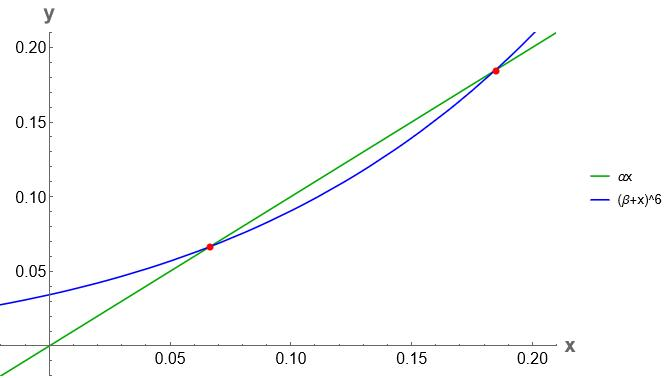
\includegraphics[width=0.5\textwidth]{deterministic/images/two_intersection.jpg}
        }
        \subfloat[\(\beta \approx 0.582355932\)]{
            \label{mainTouch}
            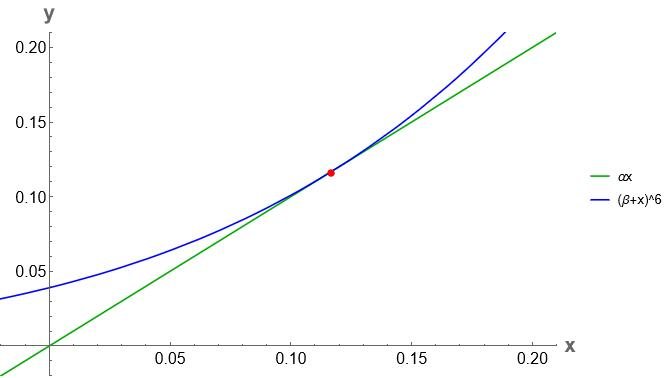
\includegraphics[width=0.5\textwidth]{deterministic/images/one_intersection.jpg}
        }

        \subfloat[\(\beta = 0.59\)]{
            \label{mainOver}
            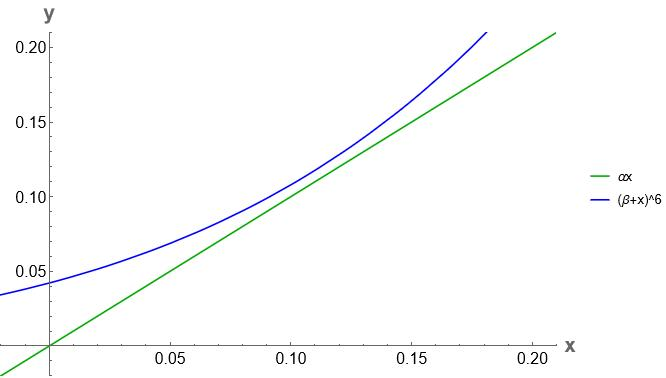
\includegraphics[width=0.5\textwidth]{deterministic/images/zero_intersection.jpg}
        } 
        % Было 0.75

        \captionsetup{justification=centering}
        \caption{Решения уравнения (\ref{baseEquation}) для разных значений параметра \(\beta\)}
    \end{figure}


    \subsection{Временные ряды}

        На временных рядах можно продемонстрировать как различные виды шума влияют на поведение системы.

        На рисунке \ref{time_series_x_0_06_a_1_b_0_56} изображено поведение модели без добавления каких-либо шумов. Видно, что значения переменной \(x\) с течением времени стабилизируются. Численность популяции фактически остается неизменной.

        \begin{figure}
            \centering
            \subfloat[Для модели (\ref{origin})]{
                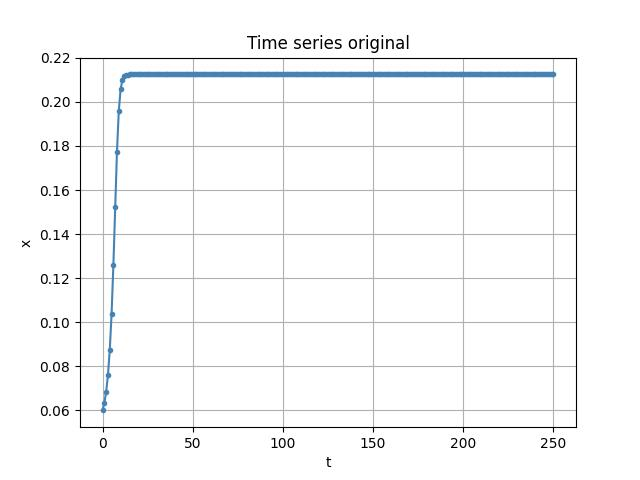
\includegraphics[width=0.5\textwidth]{stochastic/time_series_x_0_06_a_1_b_0_56.jpg}
                \label{time_series_x_0_06_a_1_b_0_56}
            }
            \subfloat[Для модели (\ref{alpha_chaos})]{
                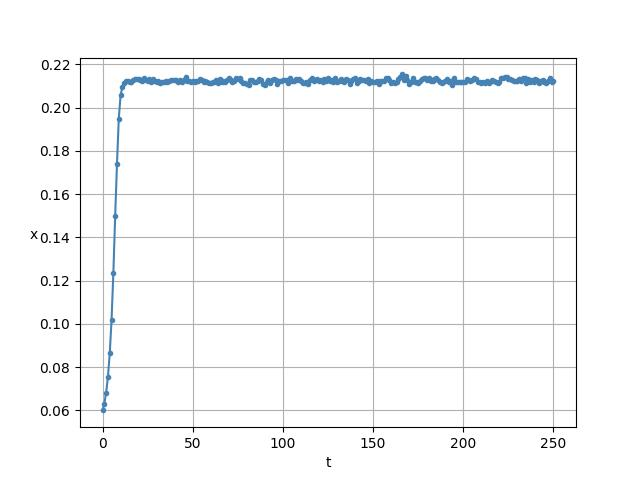
\includegraphics[width=0.5\textwidth]{stochastic/time_series_x_0_06_a_1_b_0_56_alpha_chaos_epsilon_0_004.jpg}
                \label{time_series_x_0_06_a_1_b_0_56_alpha_chaos_epsilon_0_004}
            }  

            \subfloat[Для модели (\ref{beta_chaos})]{
                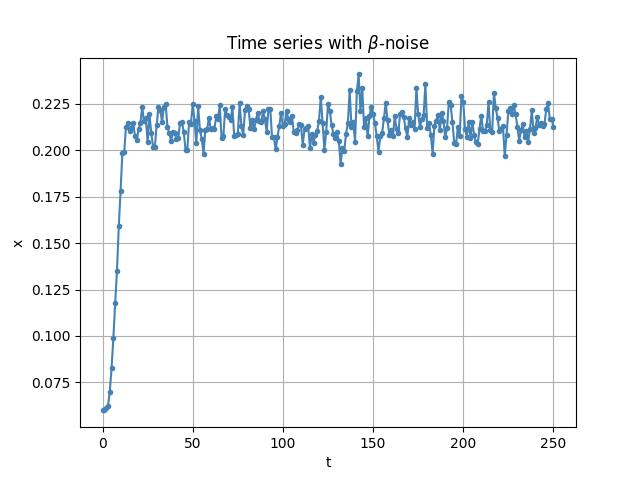
\includegraphics[width=0.5\textwidth]{stochastic/time_series_x_0_06_a_1_b_0_56_beta_chaos_epsilon_0_004.jpg}
                \label{time_series_x_0_06_a_1_b_0_56_beta_chaos_epsilon_0_004}
            }
            \subfloat[Для модели (\ref{additive_chaos})]{
                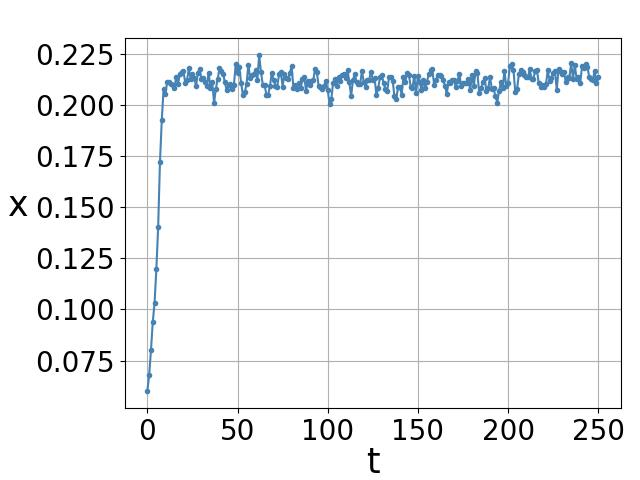
\includegraphics[width=0.5\textwidth]{stochastic/time_series_x_0_06_a_1_b_0_56_additive_chaos_epsilon_0_004.jpg}
                \label{time_series_x_0_06_a_1_b_0_56_additive_chaos_epsilon_0_004}
            }
            
            \caption{Временные ряды при \(\alpha = 1, \beta = 0.56, x_0 = 0.06, \varepsilon = 0.004\)}
        \end{figure}

        Далее на рисунках \ref{time_series_x_0_06_a_1_b_0_56_alpha_chaos_epsilon_0_004}, \ref{time_series_x_0_06_a_1_b_0_56_beta_chaos_epsilon_0_004}, \ref{time_series_x_0_06_a_1_b_0_56_additive_chaos_epsilon_0_004} представлены временные ряды для различных видов шума: 

        \begin{enumerate}[a)]
            \setcounter{enumi}{1}
            \item \(\alpha\)-шум
            \item \(\beta\)-шум
            \item аддитивный шум
        \end{enumerate}

        Все варианты рассматриваются с одной и той же интенсивностью шума \(\varepsilon = 0.004\). 
        
        Мы видим, что вид шума влияет на величину разброса значений численности популяции. \comment{Приплети сюда дисперсию.} И если раньше численность популяции стабилизировалась и переставала хоть сколько-нибудь меняться, то сейчас численность постоянно всегда колеблется, но как можно заметить, она меняется в рамках некоторого коридора значений. Численность популяции в общем то не растет и не уменьшается на какую-то значительную величину. Но такое поведение наблюдается не всегда.

        \comment{малый шум будет оказывать незначительное влияние, а большой - огромное.}

        \comment{Можно взять оригинальный временной ряд и на него сверху наложить временной ряд с шумом.}

        \comment{Хорошая фраза: индуцированный шумом переход}

        Для того чтоб продемонстрировать другое возможное поведение, давайте увеличим интенсивность шума. Пускай теперь \(\varepsilon = 0.04\). Рассмотрим рисунок \ref{time_series_x_0_06_a_1_b_0_56_beta_chaos_epsilon_0_04_fall}. Здесь мы видим ситуацию, когда шум оказал негативное влияние на численность популяции. Но опять же все не так просто. Если мы еще раз запустим алгоритм, который просчитывает нашу модель, то мы увидим, что популяция успешно выживала на протяжении анализируемого интервала времени. Данный пример проиллюстрирован на картинке \ref{time_series_x_0_06_a_1_b_0_56_beta_chaos_epsilon_0_04_alive}. Аналогичные эффекты можно наблюдать и при других видах шума.

        \comment{Примерно в \(t = 50\) обе популяции были близки к вымиранию, но одна выжила, а вторая нет. "Одно рисовое зернышко может склонить чашу весов" (с) какой-то мультик.}

        \begin{figure}
            \centering
            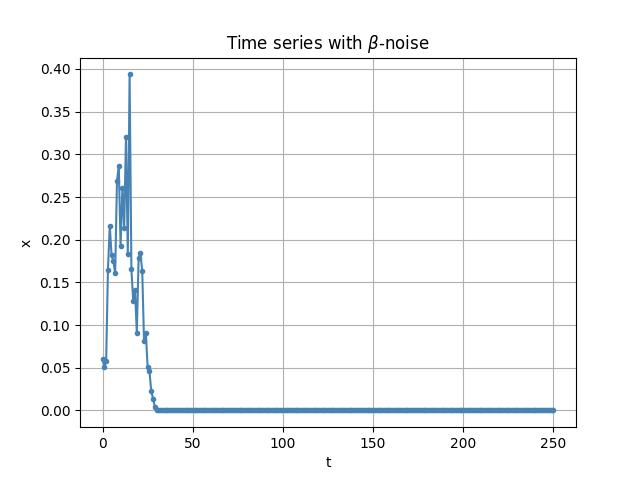
\includegraphics[width=\textwidth]{stochastic/time_series_x_0_06_a_1_b_0_56_beta_chaos_epsilon_0_04_fall.jpg}
        
            \captionsetup{justification=centering}
            \caption{Временной ряд модели (\ref{beta_chaos}) при \(\beta = 0.56, \alpha = 1, x_0 = 0.06, \varepsilon = 0.04\)}
            \label{time_series_x_0_06_a_1_b_0_56_beta_chaos_epsilon_0_04_fall}
        \end{figure}

        \begin{figure}
            \centering
            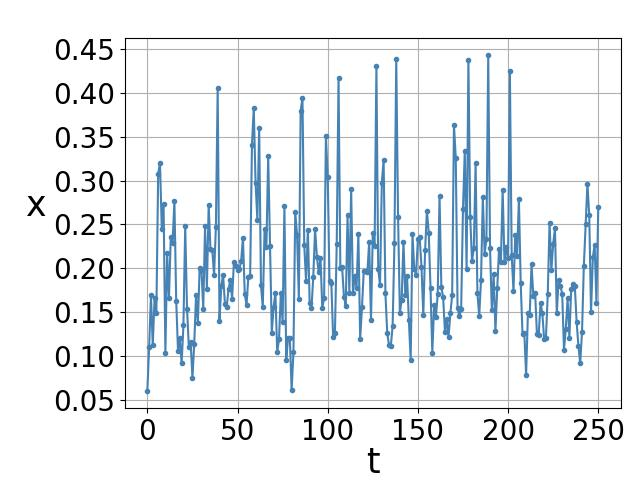
\includegraphics[width=\textwidth]{stochastic/time_series_x_0_06_a_1_b_0_56_beta_chaos_epsilon_0_04_alive.jpg}
        
            \captionsetup{justification=centering}
            \caption{Временной ряд модели (\ref{beta_chaos}) при \(\beta = 0.56, \alpha = 1, x_0 = 0.06, \varepsilon = 0.04\)}
            \label{time_series_x_0_06_a_1_b_0_56_beta_chaos_epsilon_0_04_alive}
        \end{figure}

        Анализируя вышесказанное можно сказать, что при добавлении в модель случайных событий ее поведение становится непредсказуемым. Одно незначительное изменение может кардинально повлиять на ход развития событий. 

        \comment{рассматривать как в том семестре все возможные варианты поведения системы в зависимости от начальной точки думаю не надо и так все понятно.}

    \subsection{Стохастические диаграммы}

    Далее представлено влияние случайного возмущения на бифуркационных диаграммах для разных видов шума. На рисунках \ref{bifurcation_x_0_2_a_1_compare_alpha_noise}, \ref{bifurcation_x_0_2_a_1_compare_beta_noise} и \ref{bifurcation_x_0_2_a_1_compare_additional_noise} представлены графики бифуркационных диаграмм для моделей (\ref{alpha_chaos}), (\ref{beta_chaos}) и (\ref{additive_chaos}). Во всех моделях зафиксировано значение параметра \(\alpha = 1\). На каждом графике, так же как и в исходной модели, существует участок равновесия, участки с циклами и участок с хаотическим поведением системы. От вида и интенсивности шума зависит то, насколько выделены участки с регулярной динамикой.

    Видно, что модель с \(\alpha\)-шум сохранят бифуркационную структуру лучше, чем модель с \(\beta\)-шумом и с аддитивным шумом.

    \begin{figure}
        \centering
        \subfloat[для модели (\ref{origin}) (без шума)]{
            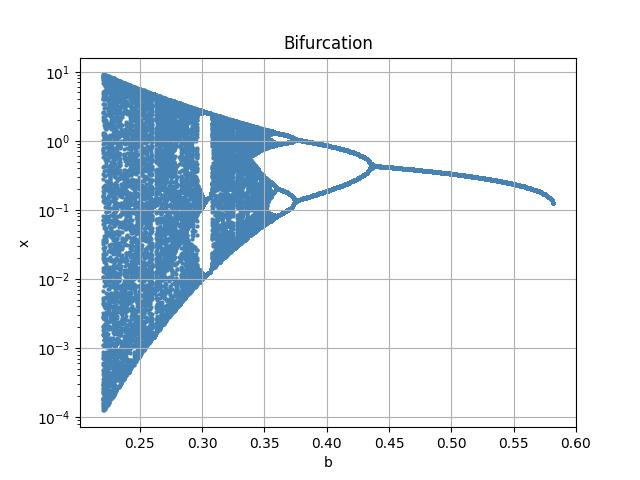
\includegraphics[width=0.55\textwidth]{stochastic/images/bifurcation_x_0_2_a_1_compare_no_noise.jpg}
            \label{bifurcation_x_0_2_a_1_compare_no_noise}
        }  
        \subfloat[для модели (\ref{alpha_chaos}) (с \(\alpha\)-шумом)]{
            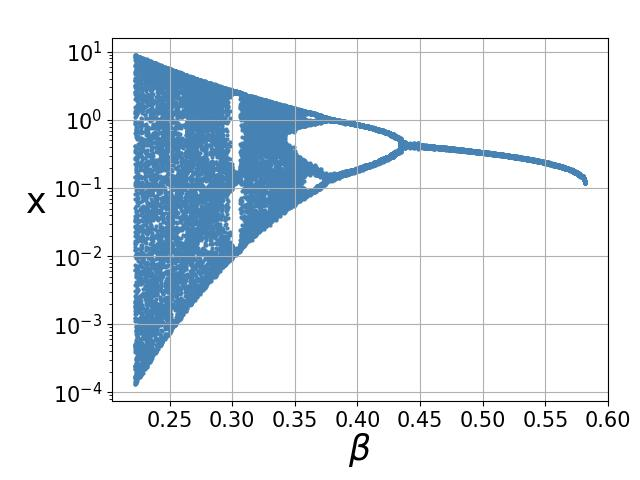
\includegraphics[width=0.55\textwidth]{stochastic/images/bifurcation_x_0_2_a_1_compare_alpha_noise.jpg}
            \label{bifurcation_x_0_2_a_1_compare_alpha_noise}
        }
        
        \subfloat[для модели (\ref{beta_chaos}) (с \(\beta\)-шумом)]{
            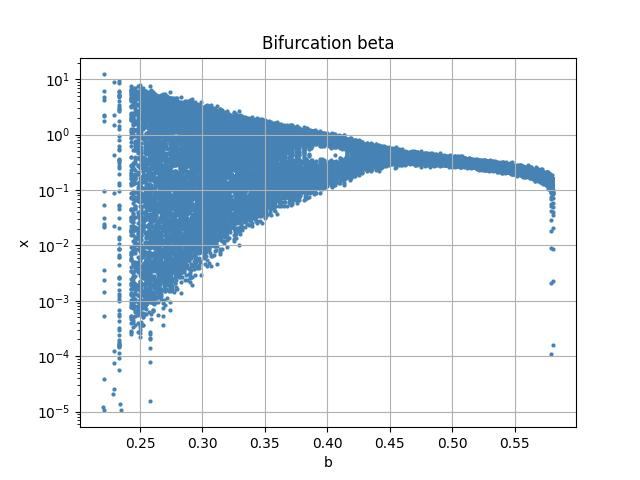
\includegraphics[width=0.55\textwidth]{stochastic/images/bifurcation_x_0_2_a_1_compare_beta_noise.jpg}
            \label{bifurcation_x_0_2_a_1_compare_beta_noise}
        }
        \subfloat[для модели (\ref{additive_chaos}) (с аддитивным шумом)]{
            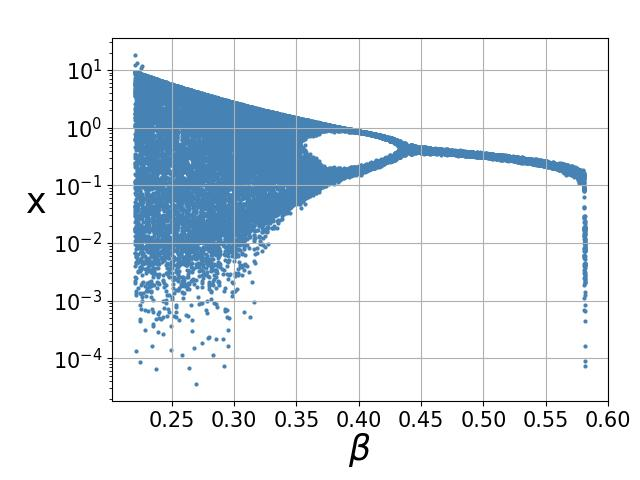
\includegraphics[width=0.55\textwidth]{stochastic/images/bifurcation_x_0_2_a_1_compare_additional_noise.jpg}
            \label{bifurcation_x_0_2_a_1_compare_additional_noise}
        }
            
        \caption{Бифуркационная диаграмма при \(\varepsilon = 0.01\)}
    \end{figure}

    % \begin{figure}
    %     \centering
    %     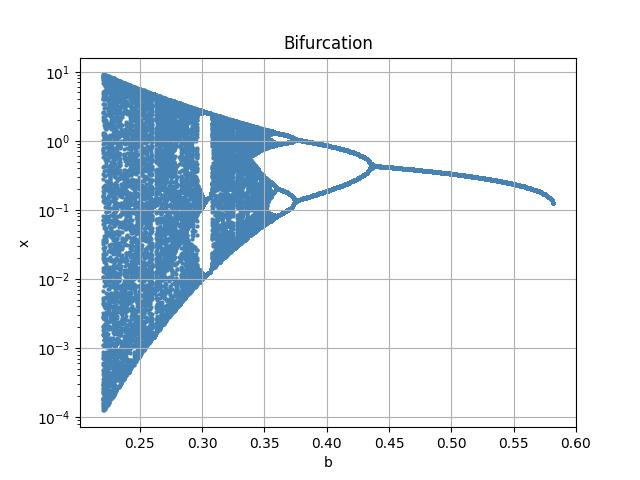
\includegraphics[width=\textwidth]{stochastic/images/bifurcation_x_0_2_a_1_compare_no_noise.jpg}
        
    %     \captionsetup{justification=centering}
    %     \caption{Бифуркационная диаграмма для модели (\ref{origin})}
    %     \label{bifurcation_x_0_2_a_1_compare_no_noise}
    % \end{figure}


    \subsection{Матожидание}

        \comment{Напиши что-нибудь про матожидание и циклическое матожидание}

        Давайте рассмотрим график матожидания \ref{EV} для модели с \(\beta\)-шумом, которая представлена формулой \ref{beta_chaos}. Мы видим, что на графике есть "выбросы" значений, например, такое можно увидеть на черной линии в точках \(\beta = 0.38\) и \(\beta = 0.45\). Для того, чтобы избавиться от таких выбросов и получить общую картинку происходящего далее будем анализировать усредненные матожидания.

        \comment{Думаю расписывать как построили усредненное матожидание не надо.}
        
        \begin{figure}
            \centering
            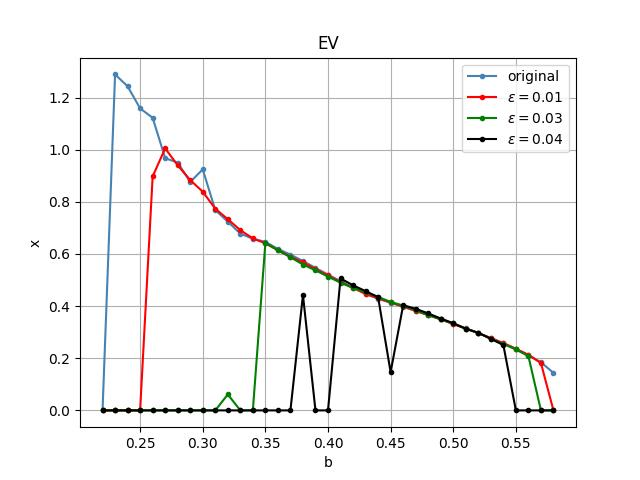
\includegraphics[width=\textwidth]{stochastic/images/EV.jpg}
        
            \captionsetup{justification=centering}
            \caption{}
            \label{EV}
        \end{figure}

        Перейдем к рассмотрению графика \ref{EV_cyclic} усредненных значений математического ожидния. Мы видим, что нам удалось избавиться от "выборосов", описанных выше. При этом можно оценить \comment{что происходит на участкх, которые уходят вниз.}
        
        \begin{figure}
            \centering
            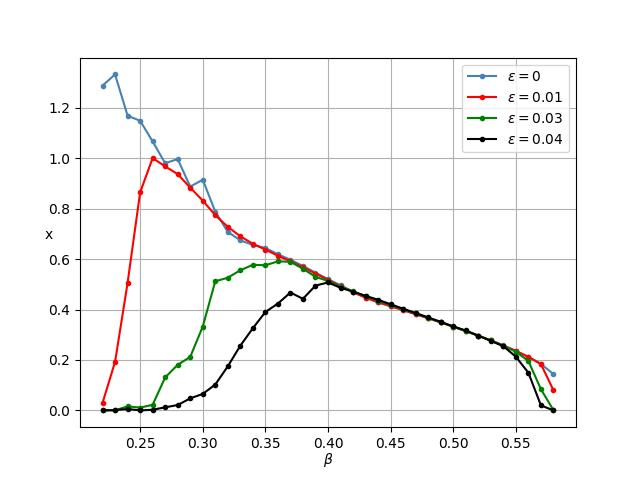
\includegraphics[width=\textwidth]{stochastic/images/EV_cyclic.jpg}
        
            \captionsetup{justification=centering}
            \caption{}
            \label{EV_cyclic}
        \end{figure}

        На графике матожидания видно, что значения бифуркации при уменьшении параметра \(\beta\) растет, доходит до какого-то значения и сваливается в ноль. Заметим также, что при увеличении интенсивности наша модель начинает уходить в ноль при более больших значениях параметра \(\beta\). Это связано с тем, что при более высокой интенсивноти, шум оказывает более сильное влияние на развитие популяции.

        \comment{При чем, если есть шум, то уходим в ноль всегда, а при остуствии шума начинается зона хаоса}

        \comment{Точка начала сваливания в ноль обусловлена траекториями...}

        \comment{Теперь про касания...}

        \comment{А разные шумы?}

    \subsection{Дисперсия}

    Для дисперсии будем строить усредненный график, аналогично тому, как мы сделали в пункте про матожидание.

    \comment{напиши что-нибудь про дисперсию и циклическую дисперсию}
        
    \begin{figure}
        \centering
        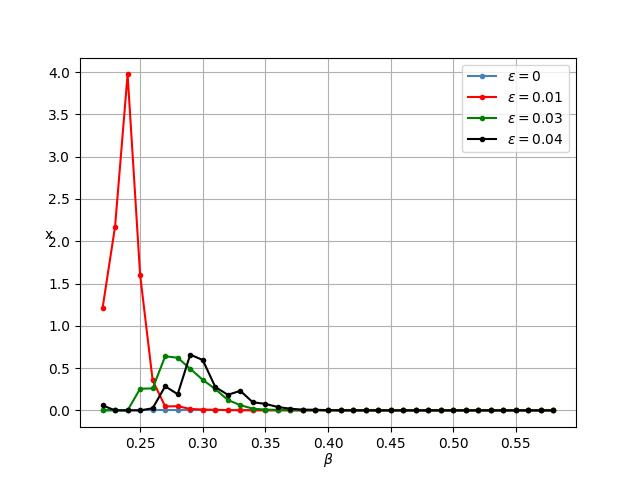
\includegraphics[width=\textwidth]{stochastic/images/variance_cyclic.jpg}
        
        \captionsetup{justification=centering}
        \caption{Дисперсия}
        \label{variance_cyclic}
    \end{figure}

    \subsection{Стохастическая чувствительность}

    Для аппроксимации вероятностного распределения случайных состояний вокруг детерминированных аттракторов (равновеися или циклов) можно использовать сетод функции стохастический чувствительности. Данный подход описан в работе Ряшко Л. Б. \cite{Ryashko}.

    На графике \ref{bifurcation_x_0_2_a_1_beta_chaos_fss} красными линиями изображена функция стохастической чувствительности. 

    \begin{figure}
        \centering
        \subfloat[Общий вид бифуркационной диаграммы с ФСЧ]{
            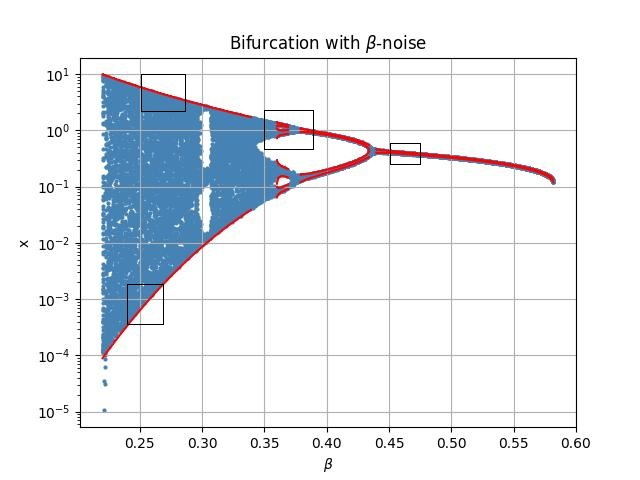
\includegraphics[width=0.7\textwidth]{stochastic/images/bifurcation_x_0_2_a_1_beta_noise_fss.jpg}
            \label{bifurcation_x_0_2_a_1_beta_chaos_fss}
        }

        \subfloat[ФСЧ для равновесия]{
            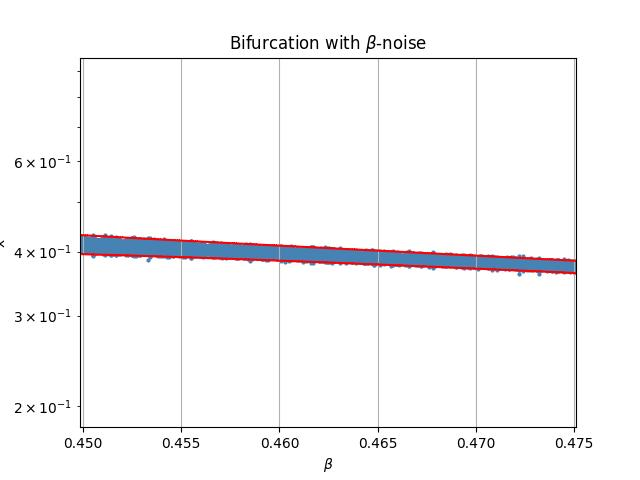
\includegraphics[width=0.5\textwidth]{stochastic/images/bifurcation_x_0_2_a_1_beta_noise_fss_segment_stable.jpg}
            \label{bifurcation_x_0_2_a_1_beta_chaos_fss_segment_stable}
        }  
        \subfloat[ФСЧ для 2-цикла]{
            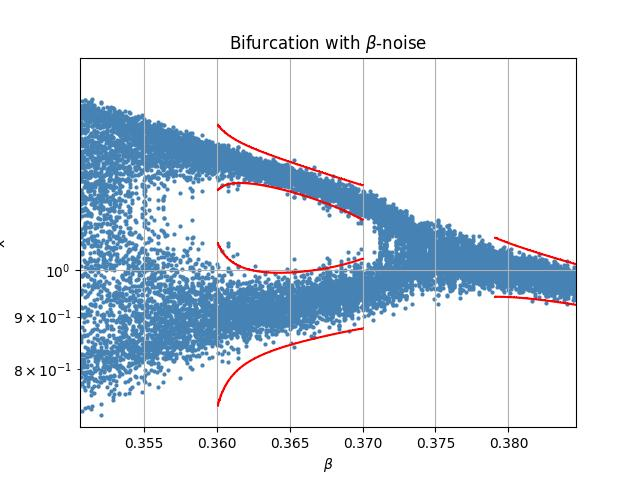
\includegraphics[width=0.5\textwidth]{stochastic/images/bifurcation_x_0_2_a_1_beta_noise_fss_segment_2_cycle.jpg}
            \label{bifurcation_x_0_2_a_1_beta_chaos_fss_segment_2_cycle}
        }
            
        \subfloat[ФСЧ для хаоса]{
            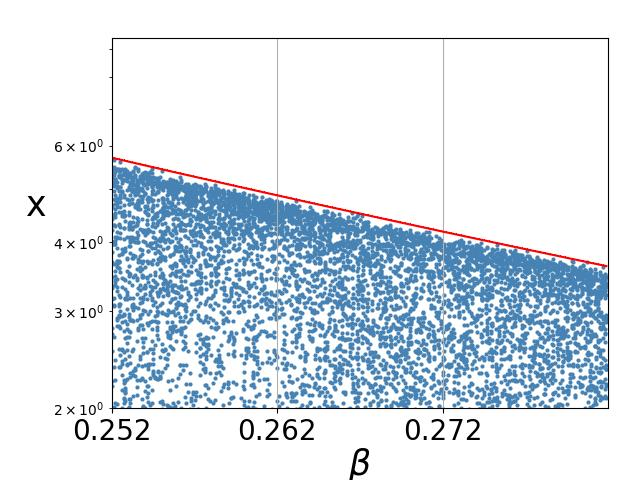
\includegraphics[width=0.5\textwidth]{stochastic/images/bifurcation_x_0_2_a_1_beta_noise_fss_segment_chaos_up.jpg}
            \label{bifurcation_x_0_2_a_1_beta_chaos_fss_segment_chaos_up}
        }
        \subfloat[ФСЧ для хаоса]{
            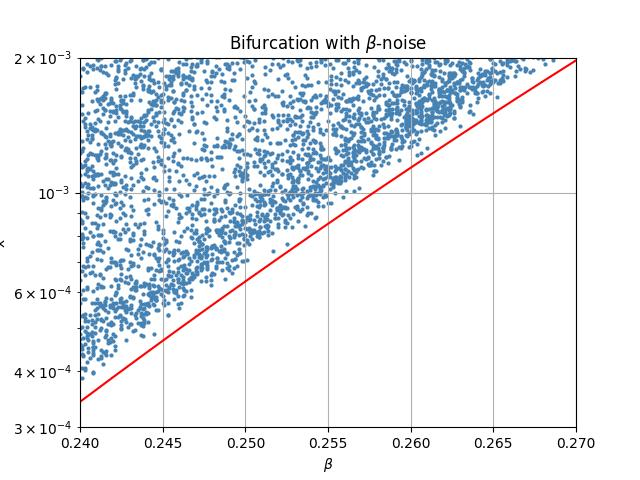
\includegraphics[width=0.5\textwidth]{stochastic/images/bifurcation_x_0_2_a_1_beta_noise_fss_segment_chaos_down.jpg}
            \label{bifurcation_x_0_2_a_1_beta_chaos_fss_segment_chaos_down}
        }
            
        \caption{Бифуркационная диаграмма с ФСЧ для модели \ref{beta_chaos}}
    \end{figure}

    Рассмотрим участок от \(\beta \approx 0.45\) до \(\beta \approx 0.48\), он изображен на рисунке \ref{bifurcation_x_0_2_a_1_beta_chaos_fss_segment_stable}. Мы видим, что значения графика бифуркации почти всегда находятся в коридоре, границами которого являются значения ФСЧ. Этот коридор строится по правилу трех сигм. Такой подход гарантирует, что почти все значения будут находиться в этом интервале, что собственно мы и наблюдаем.

    На участках с k-циклами и хаосом (рисунки \ref{bifurcation_x_0_2_a_1_beta_chaos_fss_segment_2_cycle}, \ref{bifurcation_x_0_2_a_1_beta_chaos_fss_segment_chaos_up} и \ref{bifurcation_x_0_2_a_1_beta_chaos_fss_segment_chaos_down}) будет наблюдаться аналогичная ситуация: значения лежат в коридоре, ограниченном значениями ФСЧ.


    \subsection{График ФСЧ}

        Функцию стохастический чувствительности можно изобразить еще одним способом, который наглядно представлен на рисунках \ref{} \comment{которых пока нет.}

        \comment{напиши что-нибудь про график фсч, это который m(beta)}

    \subsection{Критическая интенсивность}

    Критической интенсивностью называется такое значение интенсивности, при котором траектории могут выходить за границы аттрактора и сваливаться в ноль.

    Например, на рисунке \ref{critical_intensity_beta_noise} изображен график критической интенсивности для \(\beta\)-шума. Красным показана критическая интенсивность для границ доверительных интервалов, которые лежат ниже устойчивого равновесия. Синим - для границ, которые выше устойчивого равновесия. 

    \comment{Для 4-цикла сделать шаг меньше и подойти ближе к 2-циклу. Холмик должен получится}

    \begin{figure}
        \centering
        \subfloat[Модель (\ref{alpha_chaos})]{
            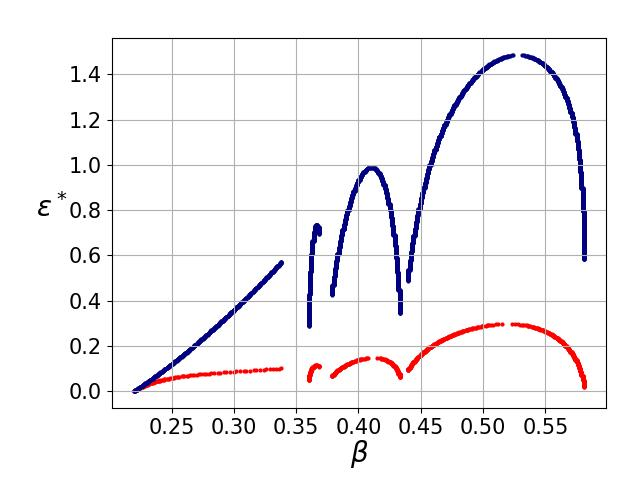
\includegraphics[width=0.55\textwidth]{stochastic/images/critical_intensity_alpha_noise.jpg}
            \label{critical_intensity_alpha_noise}
        }

        \subfloat[Модель (\ref{beta_chaos})]{
            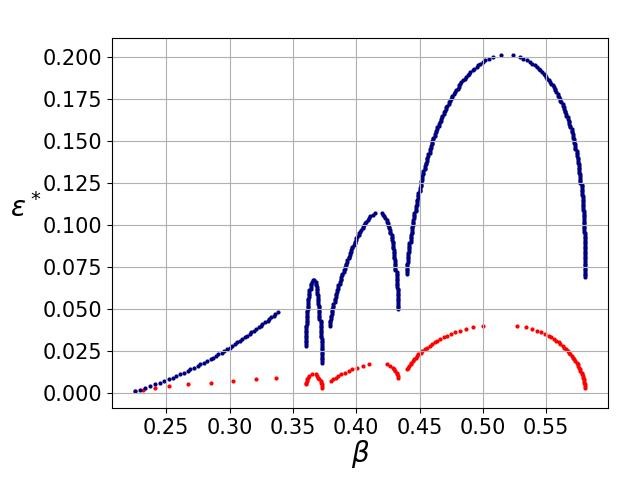
\includegraphics[width=0.55\textwidth]{stochastic/images/critical_intensity_beta_noise.jpg}
            \label{critical_intensity_beta_noise}
        }
        
        \subfloat[Модель (\ref{additive_chaos})]{
            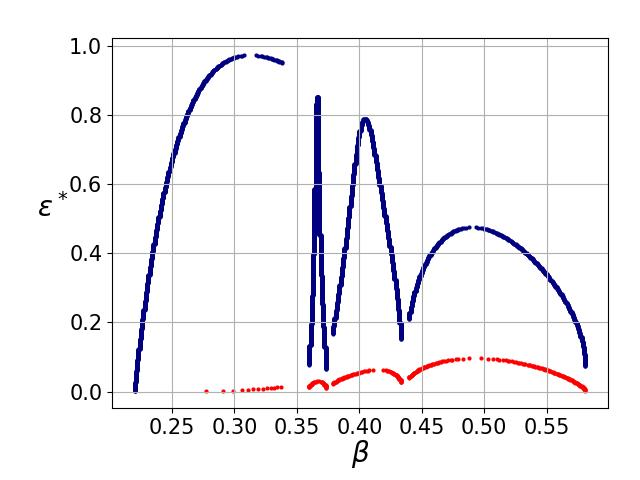
\includegraphics[width=0.55\textwidth]{stochastic/images/critical_intensity_additive_noise.jpg}
            \label{critical_intensity_additive_noise}
        }
            
        \caption{Критическая интенсивность}
    \end{figure}
    
    Обозначения аналогичны для графиков \(\alpha\)-шума (\ref{critical_intensity_alpha_noise}) и аддитивного шума (\ref{critical_intensity_additive_noise}).

    Интересно заметить, что в случае \(\alpha\)-шума и \(\beta\)-шума силуэты графиков очень похожи. В то же время график для аддитивного шума не похож на предыдущие случаи.


    \subsection{Метрика Махаланобис}

    Как было показано выше значение критической интенсивности, а знаичт и вероятности выживания попцляции зависит от двух факторов: стохастической чувствительности аттрактора и расстояния до границы бассейна притяжения. Здесь дает ответ следующая метрика. Метрика Махаланобиса показывает расстояние мжду двумя точкасм с учетом стохастической чувствительности аттрактора.

    Метрика Махаланобис рассчитывается по формуле:

    \[d_M = \frac{|x_2^* - x_1^*|}{\sqrt{M}}\]
        
    где \(x_2^*\) --- устойчивое равновесие, либо один из элементов цикла, либо граница хаотического аттрактора. \(x_1^*\) --- либо неустойчивое равновесие, либо его прообраз. \(M\) --- значение функции стохастической чувствительности.

    Графики зависимотстей метрики от параметра \(\beta\) изображены на рисунках \ref{mahalanobis_metrics_alpha_noise}, \ref{mahalanobis_metrics_beta_noise} и \ref{mahalanobis_metrics_additive_noise}

    \comment{Как связаны фсч и критическая интенсивность}

    \comment{Вставь евклидово расстояние}

    \begin{figure}
        \centering
        \subfloat[Для модели (\ref{alpha_chaos})]{
            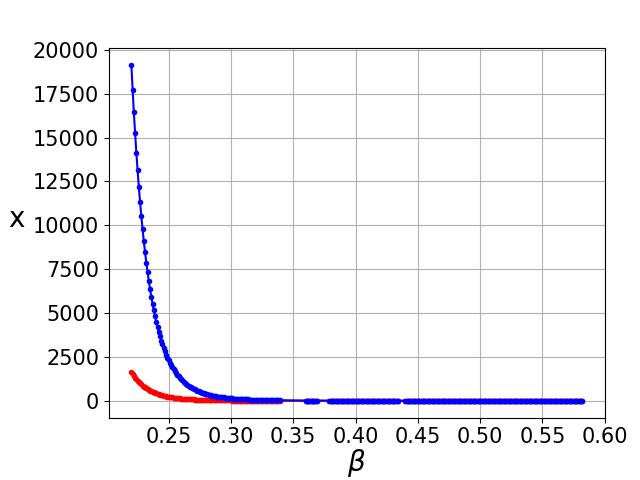
\includegraphics[width=0.55\textwidth]{stochastic/images/mahalanobis_metrics_alpha_noise.jpg}
            \label{mahalanobis_metrics_alpha_noise}
        }
        
        \subfloat[Для модели (\ref{beta_chaos})]{
            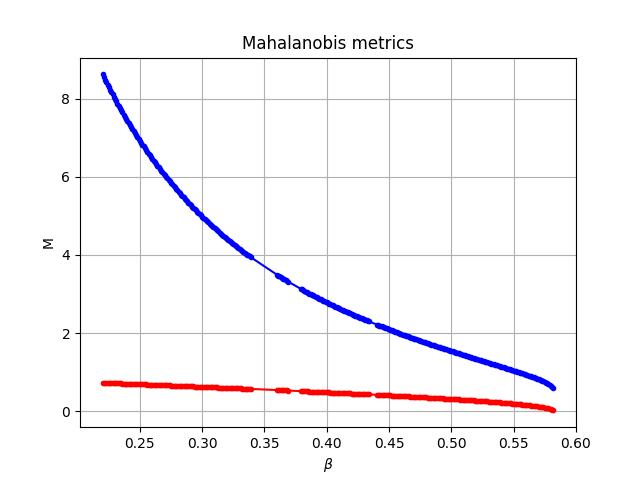
\includegraphics[width=0.55\textwidth]{stochastic/images/mahalanobis_metrics_beta_noise.jpg}
            \label{mahalanobis_metrics_beta_noise}
        }  

        \subfloat[Для модели (\ref{additive_chaos})]{
            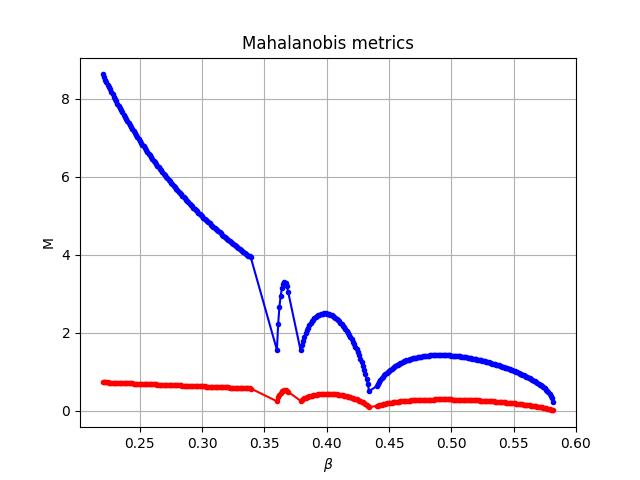
\includegraphics[width=0.55\textwidth]{stochastic/images/mahalanobis_metrics_additive_noise.jpg}
            \label{mahalanobis_metrics_additive_noise}
        }
        
        \caption{Метрика Махаланобис}
    \end{figure}
            


    \newpage

    \section{Заключение}

    В работе представлены результаты компьютерного моделирования и анализа динамики численности популяции модели Хасселя. В рамках анализа с помощью методов численного моделирования были построены временные ряды, бифуркционные диаграммы, лестница Ламерея, показатель Ляпунова. Так же были найдены и изучены зоны сосуществования устойчивых равновесий и циклов.

    Для визуализации использовались Python 3.9, mathplotlib, GeoGebra и Wolfram Mathematica. Для вычислений --- Python 3.9 и GeoGebra.

    \comment{@book{
  elementsOfNonlinearDynamic,
  author = {Ряшко, Л. Б. and Васин, В. В.},
  year = {2006},
  title = {Элементы нелинейной динамики: от порядка к хаосу}
}}

    \bibliographystyle{apalike}
    % \bibliographystyle{gost2008}
    \bibliography{main}
\end{document}